\documentclass[a4paper,landscape,9pt]{article}

\usepackage[margin=1cm]{geometry}
\usepackage{fontspec}
\setmainfont{TeX Gyre Pagella}
\usepackage{unicode-math}
\setmathfont{TeX Gyre Pagella Math}

\usepackage{tikz}
\usetikzlibrary{arrows.meta,calc,positioning,shapes.geometric}
\usepackage{microtype}

\pagestyle{empty}
\setlength{\parindent}{0pt}
\setlength{\parskip}{0.25em}

\tikzset{
  node-d/.style={draw,fill=black,regular polygon,regular polygon sides=6,minimum size=7mm,inner sep=0pt,text=white,font=\tiny\bfseries},
  node-a/.style={draw,fill=black!70,regular polygon,regular polygon sides=3,minimum size=7mm,inner sep=0pt,text=white,font=\tiny\bfseries},
  node-t/.style={draw,circle,minimum size=7mm,inner sep=0pt,line width=0.4pt,font=\tiny},
  node-o/.style={draw,fill=black!15,rectangle,minimum size=7mm,inner sep=0pt,font=\tiny},
  node-i/.style={draw,diamond,minimum size=8mm,inner sep=0pt,line width=0.4pt,font=\tiny},
  impl/.style={-{Latex[length=1.2mm]},line width=0.3pt,black!80},
  exemp/.style={-{Latex[length=1.2mm]},line width=0.3pt,dashed,black!80},
  band/.style={font=\scriptsize\scshape,text=black!60},
  bandline/.style={draw,black!18,line width=0.3pt},
}

\begin{document}

\begin{center}
{\large\scshape Proposisjonsgraf, seksjon 3}\hspace{0.8em}{\itshape Seleksjonstrykka spenner ut eit landskap}
\end{center}

\vspace{-0.6em}

\begin{center}
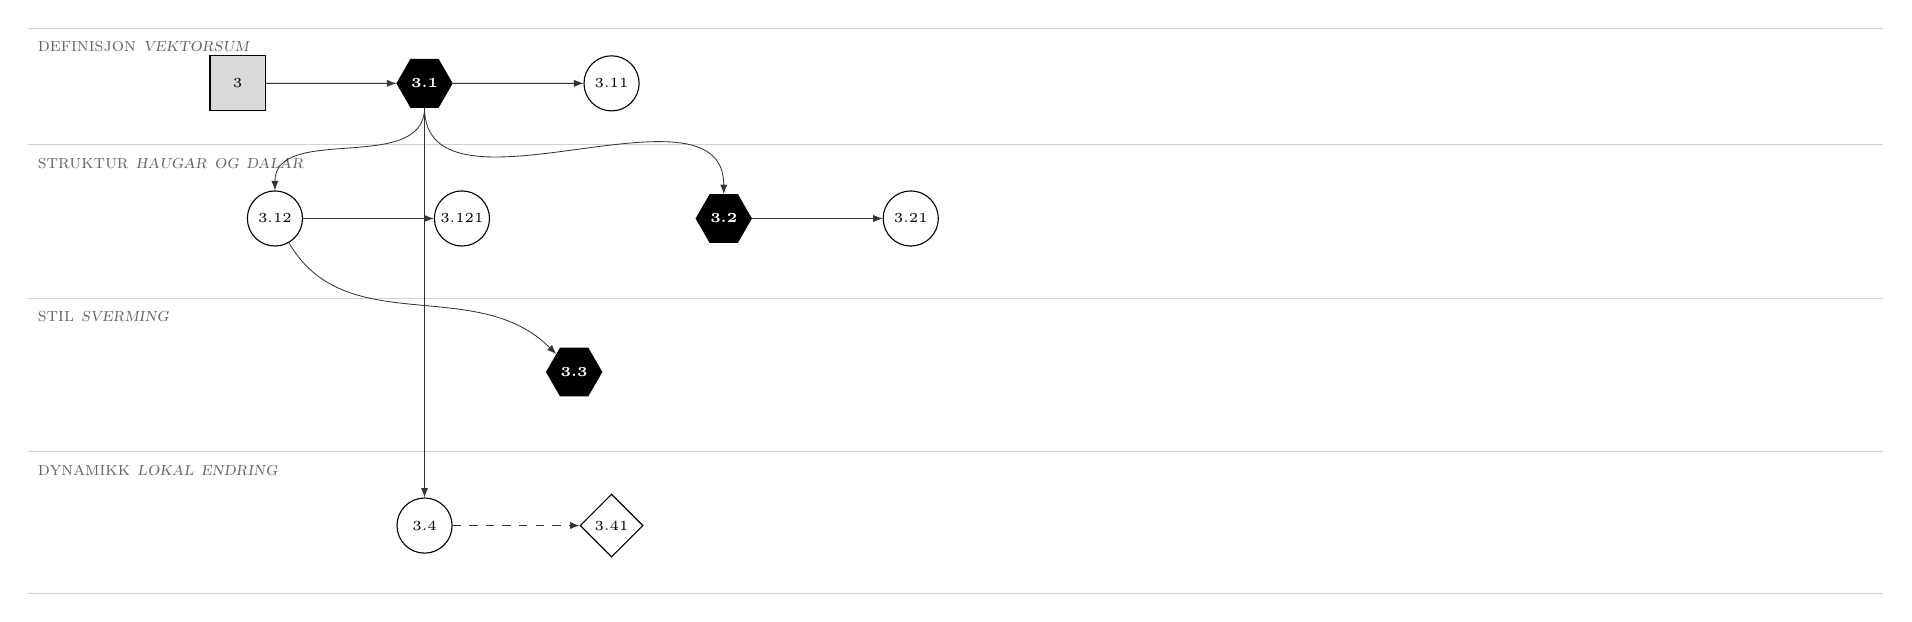
\begin{tikzpicture}[x=0.95cm,y=0.78cm]

  \draw[bandline] (-0.3, 0.6)   -- (24.5, 0.6);
  \draw[bandline] (-0.3, -1.3)  -- (24.5, -1.3);
  \draw[bandline] (-0.3, -3.8)  -- (24.5, -3.8);
  \draw[bandline] (-0.3, -6.3)  -- (24.5, -6.3);
  \draw[bandline] (-0.3, -8.6)  -- (24.5, -8.6);

  \node[band,anchor=west] at (-0.3, 0.3)  {definisjon  \itshape vektorsum};
  \node[band,anchor=west] at (-0.3, -1.6) {struktur  \itshape haugar og dalar};
  \node[band,anchor=west] at (-0.3, -4.1) {stil  \itshape sverming};
  \node[band,anchor=west] at (-0.3, -6.6) {dynamikk  \itshape lokal endring};

  % BAND 1: definisjon og epistemisk grense
  \node[node-o] (p3)      at (2.5, -0.3)  {3};
  \node[node-d] (p31)     at (5, -0.3)    {3.1};
  \node[node-t] (p311)    at (7.5, -0.3)  {3.11};
  \draw[impl] (p3)  -- (p31);
  \draw[impl] (p31) -- (p311);

  % BAND 2: struktur (topologi og stabilitet)
  \node[node-t] (p312)    at (3, -2.5)    {3.12};
  \node[node-t] (p3121)   at (5.5, -2.5)  {3.121};
  \node[node-d] (p32s)    at (9, -2.5)    {3.2};
  \node[node-t] (p321)    at (11.5, -2.5) {3.21};
  \draw[impl] (p31) to[out=-90,in=90] (p312);
  \draw[impl] (p312) -- (p3121);
  \draw[impl] (p31) to[out=-90,in=90] (p32s);
  \draw[impl] (p32s) -- (p321);

  % BAND 3: stil (sverming)
  \node[node-d] (p33)     at (7, -5)      {3.3};
  \draw[impl] (p312) to[out=-60,in=135] (p33);

  % BAND 4: dynamikk
  \node[node-t] (p34)     at (5, -7.5)    {3.4};
  \node[node-i] (p341)    at (7.5, -7.5)  {3.41};
  \draw[impl] (p31)  to[out=-90,in=90,looseness=1.2] (p34);
  \draw[exemp] (p34) -- (p341);

\end{tikzpicture}
\end{center}

\vspace{-0.2em}

\hrule

\vspace{0.4em}

\begin{minipage}[t]{0.325\textwidth}
{\scshape\small Lesing ovanfrå}

Rota \emph{3} er den knappe observasjonen at trykka spenner ut eit landskap. Band 1 gjer han presis: \emph{3.1} definerer landskapet som \textbf{vektorsum} av verksame seleksjonstrykk, og \emph{3.11} legg til ei avgjerande epistemisk avgrensing: landskapet let seg berre lodde retrospektivt.

Dette er eit viktig teorem. \emph{3.11} seier at teorien ikkje er prediktiv på einskildform; han yter berre lokal prediksjon. Hjå filosofen er dette eit sjeldan og ærleg grep.
\end{minipage}\hfill
\begin{minipage}[t]{0.325\textwidth}
{\scshape\small Lesing nedover}

Band 2 karakteriserer landskapets struktur langs to aksar. Til venstre: topologien av \textbf{lokale maksima} (\emph{3.12}) og den empiriske knusinga av den universelle toppen (\emph{3.121}). Til høgre: \textbf{stabiliteten} som funksjon av dalveggens brattleik (\emph{3.2, 3.21}). Dette er langsam kanalisering mot djupe attraktorar.

\emph{3.3} i band 3 omdefinerer \textbf{stilarten} som ein sverm kring eit tyngdepunkt; eit lokalt maksimum. Ho kviler direkte på \emph{3.12}, og indirekte på \emph{3.1} via transitivitet. Dette er ikkje ein konfluens fordi avhengigheita til \emph{3.1} er transitivt gjeven gjennom \emph{3.12}.

Band 4 opnar for dynamikken som seksjon 4 vil ta over. \emph{3.41} illustrerer: isolerte tradisjonar som navigerer same kløfta utan å utveksle eit ord.
\end{minipage}\hfill
\begin{minipage}[t]{0.325\textwidth}
{\scshape\small Strukturelle innsikter}

\emph{Ingen konfluens i streng forstand.} Hypotesa frå seksjon 1 og 2 er falsifisert. Seksjon 3 manglar syntesepunktet. Den reviderte hypotesa er: \emph{karakteriseringsseksjonar treng ikkje konfluens}.

\emph{Karakterisering framfor oppfinning.} Seksjon 3 introduserer ingen ny ontologi. Han karakteriserer landskapet som allereie vart namngjeve i seksjon 2.

\emph{Ingen postulat.} Triangla er borte att. Seksjonen tek ikkje på seg ny teoretisk risiko.

\emph{Spinne seksjonen.} Berre ti proposisjonar, mot 30+ i seksjon 1. Dette er ikkje slurv, det er presisjon: eit karakteriseringsgrep er ferdig når strukturen er teikna.

\emph{\emph{3.11} som metodologisk stolpe.} Den retrospektive klausulen hindrar rammeverket i å bli prediktiv hybris. Han er ein av dei viktigaste einskildproposisjonane i traktaten.
\end{minipage}

\end{document}
